\chapter{Background and Theory}
In this chapter, we discuss the theory underlying the core issues we are trying to tackle. We outline the concepts that make up the current state of Automated Planning, such as domains, languages, solvers and more. We then explore examples tools, learning models and solvers that have been developed to date, such as pracmln a python based Markov Logic Network learning tool, AMAN an uncertainty based approach for learning action models, ARMS a MAX-SAT based approach for learning action models, PDDL a domain language and ffx a solver. We will use the theory to draw conclusions relating to the feasibility and requirements to achieve the goals outlined in the introduction for this project.


\section{Modelling Domains}
Creating a complex system in which agents act independently of user input can be a highly complex task. An agent within such a system must generate a plan in order to define which actions are optimal given the state of the environment (Domain) in which it exists. A planner may often require knowledge of other agents within the domain in order to distribute work more effectively, for this reason a language providing the ability to model such a domain is required. Such a language also allows existing planners to solve for defined problems without knowledge of the domain. Many languages exist the most prominent of which is STRIPS. \newline
STRIPS was the name given to a component in charge of planning for the software used in Shakey the robot developed by the Stanford Research Institute. Shakey was the first machine to be able to reason about it's own actions there for a sort of ancestor to modern autonomous agents. Shakey had multiple relatively basic abilities (visual analysis, object manipulation and more), what made Shakey impressive was the ability to received a set of goals to achieve and using the STRIPS planner generate the required actions to get as close to the desired solution.
\newpage
\subsection{STRIPS}
An instance of STRIPS (Stanford Research Institute Problem Solver) can be represented as a quadruple \(\{P,O,I,G\}\)
\begin{itemize}
  \item \(P\) is a set of propositional variables (represents a given state)
  \item \(O\) is a set of operators (actions) each of which is in itself a quadruple \(p_{true},p_{false},p_{add},p_{del}\), each item representing a set of propositional variable required as a precondition (true/false) or as an effect (add/del) of an operator.
  \item \(I\) is the initial state, just like \(P\) it is a set of propositional values that are initially true.
  \item \(G\) is the goal state represented as a tuple \(\{g_{true},g_{false}\}\), each a set of propositional values that must be True or False in  order for the goal to be deemed as achieved.
\end{itemize}
A plan for a given STRIPS instance is a sequence of operators that upon execution from the initial state leads to the goal state.

\subsection{PDDL}
PDDL  (Planning Domain Definition Language) is a framework designed to standardise domain, problem and planning languages. As previously discussed, STRIPS is not the only language. PDDL was created in order to make the yearly International Planning Competition (IPC) possible. This competition evaluates the performance of proposed planning systems on a set of well known bench-marked problems, hence a standardised language for defining such problems was required. Many planners do not support the full extent of PDDL, and instead focus on the most popular requirements listed in the PDDL specification, these include (STRIPS, ADL, typing, existential preconditions,equality, conditional effects ) and more. PDDL has evolved over the years and new ever more complex releases were created in order to support the ever increasing complexity of planning tasks. PDDL 2.1 adds durative actions and inequalities and PDDL 3.0 adds prefrences and contstraints. 

An important note about planners is that they not only do not support full PDDL, but depending on the planner, there may only work correctly on a specific format. These formats can be things such as requiring action preconditions/effects to be written only as conjunctions. most planners may ignore the "requirements secion of PDDL", hence when testing a planner on a problem, one cannot assume it will work unless tested or documentation is provided.

One of the largest most up to date websites for identifying PDDL requirements and active usage is the planning.wiki website where up to date documnetation of the PDDL standard is provided.

PDDL consists of a domain file and a problem file. The PDDL domain file consists of a set domain definition types (such as actions, durative-actions, functions, axioms, requirments, types.) defined by the PDDL version in use. the PDDL Domain defines the "rules" of the world upon which a problem is defined. The problem file is made up of four components. A reference to a domain upon which the problem is based

\section{Parsers}
Parsing is important because it allows us to translate a language into another. In our case we want to simulate a PDDL Domain in python, hence we require a parser to interpret PDDL and convert it to a relevant data structure. We want to make our framework as open, modular and easy to use as possible, hence we need to be able to convert different domain languages into one python based simulator, and considering that languages evolve, so must the translation layer. Parsers are perfect for this job because they convert a formal language with specific rules using Lexical Analysis into Tokens, constructing a tree which can then be translated into a new language. Parsers are considered to be mature, most modern programming languages provide very comprehensive parsing toolkits allowing for the efficient interpretation of a language, especially if it's grammar is well defined.
% Solvers & outputs
\begin{figure}[h]
\centering
 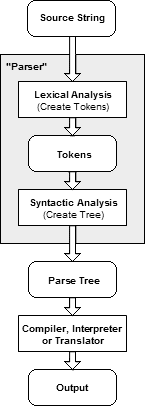
\includegraphics[height=300px]{images/architecture/parserflow}
 \caption{Parsing process architecture.}
 \label{fig:parserflow}
\end{figure}
\ref{fig:parserflow} represents a common case of a parsing flow, in this case parsing a computer language \cite{ParsingW23:online}. The first stage of the parsing process involves converting an input stream of characters into tokens (set of characters) defined by a grammar (regular expressions) written for the language being analysed. A lexer ensures that the generated tokens are meaningful by leveraging grammar defined for the language. Once tokens are generated the next stage is syntactic analysis in order to check that tokens are in the correct order and format. Grammar definitions are usually written with context-free format, which defines layers of components that can appear in the language in a recursive manner, for example, a top level component such as a book will be composed chapters, paragraphs and sentences. Syntactic analysis usually generates a tree that is then ready for parsing and interpretation. This section is what allows us to convert data in a previously cumbersome format such as text into a useful format such as a custom data structure in a given language.

Given the above specification, we can observe that writing a parser from scratch is cumbersome. For this reason most common languages today offer parsing toolkits which allow for efficient construction of parsers by taking care of the heavy lifting, meaning a developer only has to defined a grammar file for the parser to construct a tree from and a transformer to convert the tree into a desired format. Existing toolkits include ANTLR, Lark, JavaCC, SYNTAX and more, each with their advantages and disadvantages. When choosing a toolkit, we must account for cross compatibility between languages, speed, memory usage, supported features.
\newpage
\section{Solvers}

Solvers for a classical planning problem usually center around the same three requirements. A characterization of an initial state, a set of goals and a set of possible actions. Solvers are then expected to synthesize a sequence of actions that when executed in the initial state will transition the world to satisfy the goal state.

A classical planning problem is based on the following assumptions:
\begin{enumerate}
\item  The state space of the planning task is finite and fully observable.
\item Actions are deterministic and instantaneous.
\item Goal attainment is complete (not partial).
\end{enumerate}

Existing solvers are language specific, meaning that they support a specific domain language and venturing outside of this specification will break the functionality of the solver. This is important because as languages and problems evolve so must the solvers, meaning that a robust system must account for solver compatibility. As an example we can take the well known Fast Downward solver published in 2004 \cite{FastDown46:online}, since then there have been upwards of 6 iterations over the initial implementation, the most recent in 2018. 
% TODO: Solver Diagram flow.



\section{Markov Logic Networks}
As we will be implementing an action model reconstruction algorithm to demonstrate the effectiveness of development with our framework, we chose to use Markov Logic Networks for our learning model. A python package called pracmln \cite{pracmln} developed for the specific purpose of learning action models using Markov Logic Networks. This section describes the theory, advantages and disadvantages of MLN's.

The purpose of Markov Logic Networks was to efficiently handle uncertainty or noise in data by combining probability and first-order logic. Traditional first-order logic permits a compact representation of predicates forming Knowledge Bases. Probabilistic graphical models such as Bayesian Networks allow for the efficient handling of uncertainty and provide flexible and efficient querying of probabilities. Today's practical applications require both the KB's and probabilistic models to tackle situations where uncertainty such as noise is a factor. MLN's combine both probability and first-order logic, with the only restriction being that the domain must be finite. Algorithms exist for learning (or training) and inference of such networks. 

A Markov logic network consists of a first-order knowledge base where each formula has a weight attached to it. These networks can be interpreted as "simple" templates for constructing large Markov Networks while incorporating rich domain knowledge.

\subsection{Markov Networks}
Markov networks fall under the branch of Undirected Graphical Models. 
They are represented as a set of random variables forming an undirected graph that must satisfy Markov properties. Markov Networks are often compared to Bayesian Networks, however there are some key differences. Unlike Bayesian Networks, which are acyclic and directed, Markov Networks can be cyclic and are undirected. Therefore there are dependencies that Markov Networks can represent (e.g., cyclic) that Bayesian Networks cannot and vice versa (e.g., induced).
Each maximal clique in the graph has a corresponding real-valued non-negative function (so-called potential function). The values of these potential functions can be viewed as how well-correlated nodes are within the clique.

Given an undirected graph \(G = (V,E)\) , V being vertices, E being edges.
A set of random variables \(X = (X_v)_{v\in V}\) form a Markov random field with respect to \(G\) if they satisfy the following three Markov properties \cite{Markovra75:online}:
\begin{enumerate}
\item Pairwise Markov property: Conditional independence of any two non-adjacent variables given all variables: \[X_u \perp\!\!\!\perp X_v \mid X_{V\setminus\{u,v\}}\]
\item Local Markov property: Conditional independence of a variable to all other variables given its neighbors: \[ X_v \perp \!\!\!\perp X_{V\setminus N[v]} \mid X_{N(v)}\] \(N(v)\)  is the set of neighbors of \(v\). \newline\(N[v] = v\cup N(v)\) representing the closed neighbourhood of \(v\).
\item Global Markov property: Conditional independence of any two subsets given a separating subset.
\[X_A \perp \!\!\!\perp X_B \mid X_S \]Separating subset meaning that any path linking nodes from \(X_A\) to \(X_B\) must pass through \(X_S\) the separating subset.
\end{enumerate}

In Bayesian Networks, the chain rule is used to build joint distributions from conditional probability distributions. Hence the use of conditional probability tables (CPD's) in order to facilitate computation of a specific query on the graph. In the case of Markov Networks we wish to calculate the potential value between two connected nodes. This is a real number as opposed to a probability between 1 and 0 as in Bayesian Networks. For Markov Networks a factor is assigned for each maximal clique which is then used to determine the probabilities of variables given a Network state.
To calculate the joint distribution of a Markov Network, the following formula is used: \[P(X=x) = \frac{1}{Z}\prod_k \phi_k(x_{\{k\}})\]
\(x_k\) is the state of variables appearing in the \(k^{th}\) clique.
\(Z\) the partition function defined as \(Z=\sum_{x\in X}\prod_k \phi\_k(x_{\{k\}})\)
\cite{mlj05pdf51:online}
\subsection{First-Order Logic (KB)}
A first-order logic knowledge base is a set of formulas written in first order logic which represent facts (hard constraints) on a set of possible worlds. Any world violating any of the constraints would be considered as having 0 probability of existence. 

Sentences in a first-order KB are constructed using four types: functions, predicates, variables and constants. Functions return a variable or a boolean e.g. divides(x,3) would return true if x is a multiple of 3. Predicates are a combination of two terms forming a relationship e.g. red house. Variables are variables as in any programming languages, they are a  placeholder for anything in a domain e.g. x representing numbers as seen in the Functions definition or the function itself. Constants are what what variables would hold at any given point during an operation, this can be any form of data such as a number or a string e.g. 1, house_1, 2 . 

First-order logic KB's allow us to do inference. The most common common representation is in the form of Horn clauses (contain at most one positive literal) this allows programming languages such a Prolog to search for statements taht hold in the KB.

\subsection{Markov Logic Networks}
The basis of MLN's is to build on first-order KB's by softening the effect of a constraint of the viability of a given world. Instead of stating a world is impossible if a constraint is not satisfied, we simply lower the likely-hood of the world by reducing the value of said constraint. Hence each formula in a MLN KB has a weight reflecting the strength of the constraint. The greater the weight of a constraint the greater the difference in log probability between a world that satisfies said constraint and one that does not (everything else remaining equal). 
\newpage
\section{Evaluating Models}
So far we have explored relevant theory behind all of the basic building blocks that will be used in the formulation of our framework except for the techniques used for evaluating action models, which will be an output of training. Evaluation of a learned model can be implementation specific, such as evaluating for performance under different but relevant conditions such as noisy, real or simulated environments. However we will go over the standard evaluation metrics for a learned model that apply most if not all modern ML situations. Before even training a model a the data used for training is split into training, testing and validation subsets typically in the 60/20/20 percentage range in order enable evaluation in later stages. Using these subsets of data, many evaluation metrics can be derived depending on the type of model being trained. In the general case for our framework we can say that our model falls under the classification type. We are creating a model that predicts an action which is not a quantitative value. For classification type models, the main metrics for evaluation are accuracy, precision and recall. As with all models, we must also look at the bias/variance trade-off metrics to ensure proper fit.

Accuracy is defined by the percentage of correct predictions on the test dataset by the model. \[ \text{accuracy} = \frac{\text{correct predictions}}{\text{all predictions}}\]

Precision is the probability that a prediction by the model is correct.
 \[ \text{precision} = \frac{\text{true positives}}{\text{false positives}+\text{true positives}}\]

Recall is calculated with respect to a class. It is the number of correct predictions for a class divided by the total number of elements that truly belong to the class.
\[ \text{recall} = \frac{\text{true positives}}{\text{true positives}+\text{false negatives}}\]

Accuracy alone is not good enough for evaluating the usefulness of prediction models as many cases exist where we are interested in predicting a class which represents a small subset of data such as disease. A model can be 90\%+ accurate by simply predicting nobody has said disease however it is useless when trying to identify people who are ill. For this reason, precision and recall provide the relevant metrics to identify the usefulness of a model. Commonly these two metrics are combined to for the f-score.
\[F_{b}=(1+b^2)\frac{\text{precision}*\text{recall}}{b^2*\text{precision}+\text{recall}}\]

\(b\) is a variable used to control the precision/recall trade-off, \(b\)<1 places more weight on precision whilst if it is greater than one recall becomes more important. When we want to ensure that all potential true samples are predicted, it is best to have a \(b\) > 1 as we want to maximize recall, precision can then be improved by subsequent analysis perhaps performed by humans, such as recognising cancer in images, or identifying people susceptible to suicide.

A model is trained on sample data hence it must generalize the knowledge learnt to some degree in order to make predictions on new samples. When a model is being trained on sample data, it attempts to fit the data to some degree, if a mode fits the training data too well, we say there is a high degree of variance as it places too much weight on individual data points, this means the model has been over-fit. On the other hand if not enough weight is placed on data points then there is high bias and a model is under-fit, an example of under-fitting would be approximating an exponential with a straight line. 
\begin{figure}[h]
\centering
 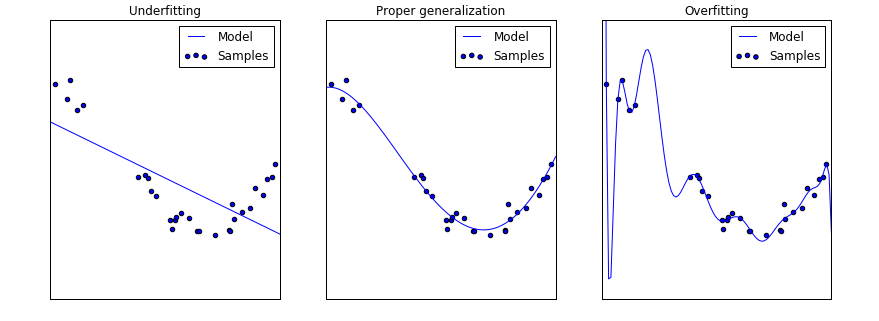
\includegraphics[width=\linewidth]{images/Selection_019}
 \caption{Bias vs Variance tradeoff.}
 \label{fig:bvtradeoff}
\end{figure}

Various tools exist for any framework when training a model in order to optimize this trade-off. A simple brute force approach involves performing a grid search by training a model multiple times with different hyper parameters. The hyper parameters that output the lowest mean square error would be the most optimal choice. Of course with more complex models and increasing number of hyper parameters, finding the optimal mean square error becomes more complex, which is why frameworks provide relevant tools for existing models. 

\newpage

\section{Existing work}\label{background:Existing Work}
We deem it important to review currently developed frameworks, learning models, and tools created by the community in order to ensure that we maximize what has already been developed by using what is available for our proof of concept implementation. there is no need to develop certain framework modules from scratch if we can tweak existing open source projects to our advantage and integrate them into our framework in order to demonstrate the flexibility and use-fullness of our design approach. 

We will review existing work associated with the five main targets outlined in our introduction in order to make sure that the work we review is closely associated with the problems we need to solve to make the framework a viable tool for development. 

\subsection{Support for various domain languages in python}
We discussed the reasons for providing support for domain languages in a higher level language, these including higher adoption rate by new developers, better legibility and compatibility with popular tools developed today. What is meant by support for a domain language in python, is essentially converting a language definition file into a well defined and tested python data structure. This data structure can then be manipulated and improved with ease as more languages are supported and tooling is improved.

Our main focus for this section is the conversion of PDDL to python. PDDL is one of the most popular planning languages today and python is the most popular programming language, which are the two most crucial factors influencing our choice. As python is so popular, multiple attempts have been conducted over the past few years to construct a PDDL parser based in python. We will provide a basic overview of the three most prominent open-source projects.

Pypddl-translator \cite{ssardina20:online} is a domain and problem PDDL parser written in python3 using PLY (Python Lex-Yacc) a parsing library. We decided to avoid this implementation due to a lack of testing, legibility and documentation. PDDL Supported functionality is defined, unfortunately errors were encountered when attempting to parse valid files due to poor coverage of PDDL requirements. PLY is also not a very popular parsing toolkit and is not as cross compatible with other languages as we would like to to be. For these reasons we have avoided inheriting from this project.

Pddl-lib \cite{hfoffani23:online} is a PDDL library that parses PDDL files using ANTLR4 grammar. It then exposes an API supporting Python 3.8. This API provides methods for obtaining the initial state, goals, operators, positive and negative preconditions as well as grounded states. This is the most sound implementation to date in python, however unfortunately it suffers of poor documentation and lack of testing. Few contributors have actively created pull requests for issues, however these have been ignored over several months. There is also no clear documentation of what has been implemented to date (supported version of PDDL and requirmenets). This makes continued development of the project difficult. Finally, the organization of resources is problematic as elements which should be separated are clumped into the same files, and contain no reference to the official PDDL paper \cite{httpsarx9:online}. Although the grammar used for parsing is popular and cross-compatible with many languages, the grammar file defined in the project lacks design definition, meaning without thorough investigation, it is very difficult to contribute to such a project without redesigning a large portion.

The last library we have reviewed is pddl-parser \cite{pucrsaut37:online}. This project conforms to modern development standards, ensuring builds are passing before merging new branches. Unfortunately  not parsing toolkit was used, instead files are parsed using python. Although for single use implementation this is ok, when a language expands or changes, these types of implementations often break as they assume a certain structure. Such an implementation is also difficult to test, modify and improve as code is much more illegible than standard parsing grammar.
Syntactic analysis is also done on the fly rather than from a tree which means any changes to the data structure that we wish to convert the parse tree to is borderline impossible. Finally such an implementation blockades use of the parser with python alone whilst most Parsing grammars offer integration with almost all modern languages.

In conclusion there is unfortunately no serious project currently being developed for parsing PDDL files, most implementation currently used in research and industry are custom and integrated directly with popular solvers making it difficult to integrate with. Hence the decision has been made to develop a formal parser for the PDDL 2.1 definition language. Design and initial implementation will be discussed further chapters.  

\subsection{Synthetic generation of training data}
Over the years many standard problems have been modeled in the planning community. Problems are usually catered to a specific level of complexity in order to allow researchers to accurately evaluate and compare new methods to existing ones. The most prominent issuer of such problems has been the IPC (International Planning Competition) which has been running since 1998 when Drew McDermott and a committee first created PDDL along with a collection of problems which defined the first benchmarks. Since then, every two years the series continued to progress with ever more difficult problems. These problems are released with a domain definition file and a generator which creates any number of goal states provided some hyper parameters. Planners are then bench-marked by their speed and ability to find optimal solutions for these problems. Well known problems include Blocksworld, Briefcaseworld, Gripper and Grid. 

What we have observed is that there is no lack of problems and generators for the acquisition of synthetic data, however it cannot be said that the process of doing so is straight forward. The most prevailing issues observed include lack of specification for execution of generators, meaning a user must find the correct compiler usually a version of C or C++ before usage. Common lack of documentation forces the user to guess what the hyper-parameters and their effects are, and finally, collecting these generators is often not very easy, as public pages are often moved, unavailable and resources are placed in archives that may not be easily accessible without spending time finding them. For these reasons we believe that collecting and providing simple wrappers for data generation over these generators in our framework will be an attractive solution saving time and effort to end users providing them better access to available resources.

Having control over what problem generators we include also allows us to set minimum standards that must be adhered to by these generators, such as standardized output and well defined language support ensuring that provided planners only execute on compatible data.



\subsection{Simplified implementation of learning models}
There has been a lot of work done in development of learning models using ever more modern techniques. However very if any work has been don in making the development of such models easier and more streamlined, making architecture of an algorithm the sole focus of research rather than being preoccupied with "support" code which is often cumbersome to implement and contributes little to research. Lets take a recent paper "Learning Action Models from Plan Traces with Disordered Actions, Parallel Actions, Noisy States"\cite{AAAIPres94:online}, we can observe that the paper bases it's tests on a relatively old and rather simple domains, as well as placing a large focus on data generation and testing it also compares results only to papers released by the same author. In comparison take "Learning STRIPS Operators from Noisy and Incomplete Observations" \cite{1210488932:online}, unlike the previous paper, the focus is not reconstructing an action model but reconstructing a network as accurately as possible, we observe that the domains used are much more complex and modern and libraries such as Tensorflow are used. Testing is also standardised and much more precise. 

The difference between both papers is the dependence on a formal domain language, the latter not being preoccupied with a specific version of PDDL or reconstructing action models for it. This demonstrates that in order for faster progress to be made, this hurdle must be tackled and dependence on underlying languages must be abstracted. Doing so will allow us to standardise certain necessities such as the reconstruction of a model output into an working action model or generation of data required for training.



\subsection{Extendable modules for conversion of training output to a standard action model}
Very little work has been done on the reconstruction of an action model. Current implementations focus on predicting the precondition, adding and deleting lists which are sub-components of an action model. These predictions are usually evaluated for error and only then are they used to rebuild an action model, however this part is usually manual. Unfortunately it is difficult to generalise the process of rebuilding an action model as the output of any learning method can be different, meaning that without a standardising the output of learning models, reconstruction is left to the designer. What we propose however is that with the accumulation of different learning models eventually many techniques for reconstruction will become available meaning learning models can cater their output to an existing reconstruction technique.

\subsection{Testing learned action models}
The issues concerning the reconstruction of action models spill over to testing of learned action models. Due to the difficult nature of reconstruction an action model, testing is usually performed directly on the output data which is vastly different from a complete action model. Such data is usually made up of predicates defining add lists or delete lists. The main issue with testing learned action models is the evaluation of similarity between it and the original model. Due to the flexible nature of language, a similarly looking (textual similarity) action model can have huge behavioral differences and vice versa. Hence it is important to identify the correct metrics for testing, especially when there are real world implications. We also must remember that as a model we are trying to learn becomes more complex and tends towards learning solely from real world data, edge cases are amongst the most difficult to learn and test due to their sparse nature. For this reason it is important to be able to simulate learned models on such cases to ensure compliance with these scenarios. This has all to often been ignored due the difficulty in setting up such a system for the sole purpose of testing a newly developed technique.
